\documentclass[12pt,titlepage]{article}
\usepackage[a4paper]{geometry}
\geometry{verbose,tmargin=2cm,bmargin=2cm,lmargin=2cm}
\usepackage[T1]{fontenc}
%\usepackage[latin2]{inputenc}%for compiling under linux uncomment line 5 and comment line 6 out. 
\usepackage[cp1250]{inputenc}
%\usepackage{polski}
\usepackage{graphicx}
\usepackage{hyperref}
\usepackage{fancyvrb}
\title{\textbf{AVR-lab01}}
\author{Krzysztof Grzes�o}
\date{}
\begin{document}
\maketitle
%\thispagestyle{empty}
%\newpage
\tableofcontents
\pagebreak
\section{Idea of the project}
Here I would like to describe the idea of the project. See sample source code of the file test.asm as described in \cite{jdoe}\\
\fvset{frame=lines,numbers=left}
%\fvset{gobble=2,numbers=left,numbersep=3pt}
\begin{Verbatim}
.include "m8def.inc"
.equ TABLE_BEGIN = 0x00
Initialization:
	; stack pointer initialization
	ldi R17, high(RAMEND)
	ldi R16, low(RAMEND)
	out SPH, R17
	out SPL, R16
	;set port A as output
	ldi R16, 0xFF
	out DDRA, R16
	ldi R30, low(Table<<1) ;save LSB of the Table address
	ldi R31, 8 ; offset set to 9th character (end of the table)
	add R30, R31
	ldi R31, high(Table<<1) ;save MSB of the Table address
	mov R19, R30 ; save table offset
	rjmp Loop

Back:
	mov R30, R19 ; set the initial offset to the table
Loop:
	lpm R18, Z ; load to program memory
	tst R18 ; check if R18 does not have TABLE_BEGIN 
	breq Back ; if so return the initial table offset
	out PORTA, R18 ; if not then display table content
	dec R30 ; and decrement pointer in a table
	rjmp Petla

Table: .DB TABLE_BEGIN, 0xFE, 0xFD, 0xFB, 0xF7, 0xEF, 0xDF, 0xBF, 0x7F
	; at the beginning of the table there is value 0x00 that would 
	; point to the initial table offset
\end{Verbatim}
\section{Schematics}
\begin{center}
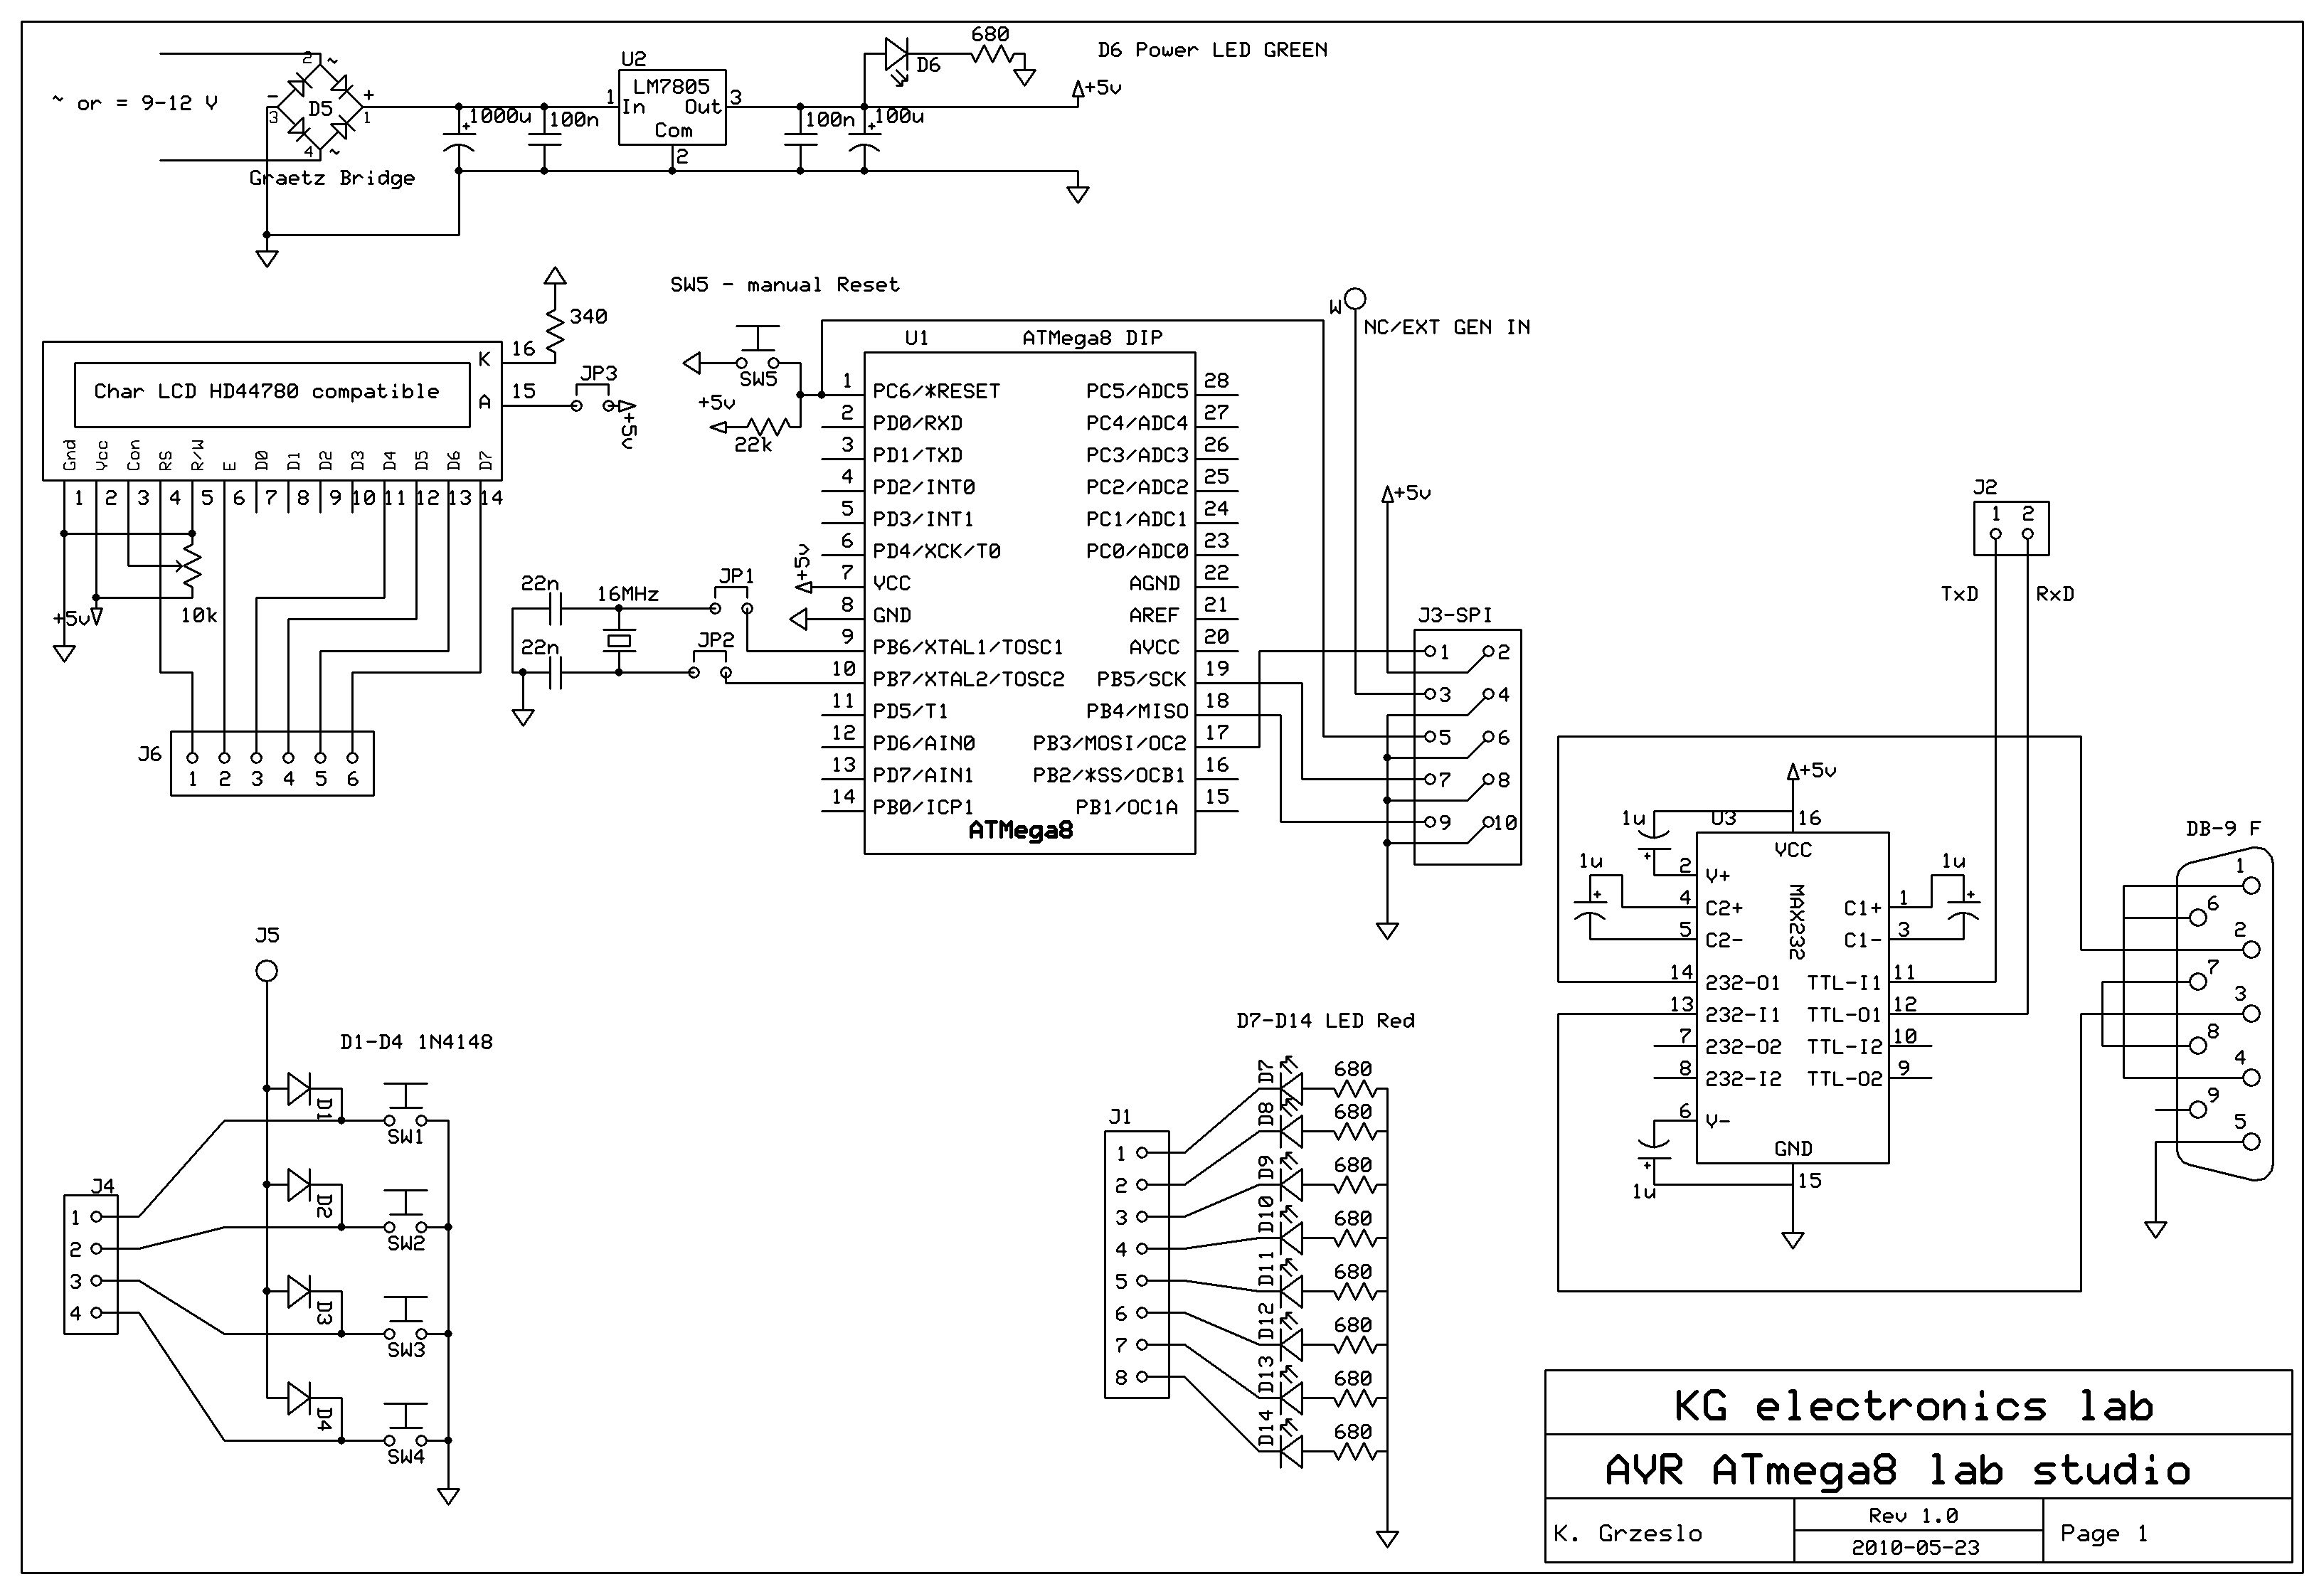
\includegraphics[height=160mm,angle=90]{../kg_avr_atmega8_lab.jpg}
\end{center}
\begin{thebibliography}{99}
\addcontentsline{toc}{section}{References}
\bibitem{jdoe} J.~Doe:
\emph{Title}, 1st Edition,
ISBN XX-XXXXX-XX-X, JDoe Editions, Imagineland 2010.

\end{document}
